% Texcount ignores the longtables
%TC:group longtable 0 0

\chapter{Testing and evaluation}\label{ch:testing-and-evaluation}
Using the implemented solution from Chapter~\ref{ch:implementation-of-the-solution} to test and evaluate its
effectiveness, both functional unit tests and agent training evaluation have been designed. To confirm that the
environment and agents implemented in the previous chapter
(section~\ref{sec:implementing-auction-and-resource-allocation-agents}) works as intended, unit testing has been added
that is explained in Section~\ref{sec:functional-testing}. While to evaluate the effectiveness of the proposed
solution from Section~\ref{sec:proposed-agents}, a range of metric have been measured during training in order to
test and compare implemented agents, neural network architectures and training parameters. These results are explained
in Section~\ref{sec:agent-evaluation}.

\section{Functional testing}\label{sec:functional-testing}
To confirm that the implementation of the agents and environment correctly, PyTest a module within Python has been used
to design functions are valid. These tests are split into three families: agent, environment and training that are
explained in the respective tables~\ref{tab:agent_testing},~\ref{tab:env_testing} and~\ref{tab:training_testing}.
The results from the testing is shown in figure~\ref{fig:pytest_results}.

\begin{longtable}{|p{3cm}|p{11cm}|} \hline
    \textbf{Test name} & \textbf{Explanation} \\ \hline
    Building agents & Constructs all of the agents with possible arguments to confirm agents can accept of all its
        attributes\\ \hline
    Saving agents & Confirms that agents can successfully save their neural networks and can successfully load
        the network again and is equal to the agent network. \\ \hline
    Agent actions & Confirms that all agents can generate valid actions for both bidding and weighting \\ \hline
    Gin config file & Gin is used to set the arguments used during training, to confirm that the file is valid. \\ \hline
    Building networks & Constructs all of the neural networks to confirm that the network return a valid output. \\ \hline
    Agent epsilon policy & While training, some of the agent actions are randomly selected to train the agents over
        a large area of the state. This tests that the random actions selected are valid. \\ \hline
    \caption{Table of test functions of the agents}
    \label{tab:agent_testing}
\end{longtable}

\begin{longtable}{|p{3cm}|p{11cm}|} \hline
    \textbf{Testing name} & \textbf{Explanation} \\ \hline
    Saving and loading an environment & The environment allows for the saving the environment at its current
        state. This tests that the environment can save and reload the environment successfully. \\ \hline
    Loading environment settings & Tests that the load environment settings correctly generates a new random
        environment based on the settings. \\ \hline
    Random action environment steps & Tests that inputs to the auction and resource allocation steps work,
        random actions are generated to check for environment edge cases.  \\ \hline
    Auction step & To confirm the Vickrey auction mechanism is completely implemented, a range of possible inputs
        are tested to confirm that right price and server that the task is allocated. \\ \hline
    Resource allocation step & To confirm that servers allocate their resources correct given some inputs. \\ \hline
    Allocation of computational resources & Checks that the server correctly allocates computational resources to
        allocated tasks. \\ \hline
    Allocation of storage and bandwidth resources & Checks that the server correctly allocates storage and
        bandwidth resources to allocated tasks. \\ \hline
    Allocation of all resources & Checks that resources are allocated by the server correctly for all of the
        resources. \\ \hline
    \caption{Table of test functions of the environment}
    \label{tab:env_testing}
\end{longtable}

\begin{longtable}{|p{3cm}|p{11cm}|} \hline
    \textbf{Testing name} & \textbf{Explanation} \\ \hline
    Task pricing training & Tests that the task pricing reinforcement learning agents can correctly learning from
        different auction observations. \\ \hline
    Resource allocation training & Tests that resource allocation reinforcement learning agents can correctly
        learn from different resource allocation observations. \\ \hline
    Agent evaluation & Tests that the agent evaluation function during training correctly captures the correct
        information due to the actions taken. \\ \hline
    Agent training & Tests that agents can be correctly trained over an environment with different actions and
        observations. \\ \hline
    Random actions training & Tests that agents with random actions can quickly using the environment training
        methods to confirm that the function work as intended. \\ \hline
    \caption{Table of test functions of agent training}
    \label{tab:training_testing}
\end{longtable}

\begin{figure}[H]
    \centering
    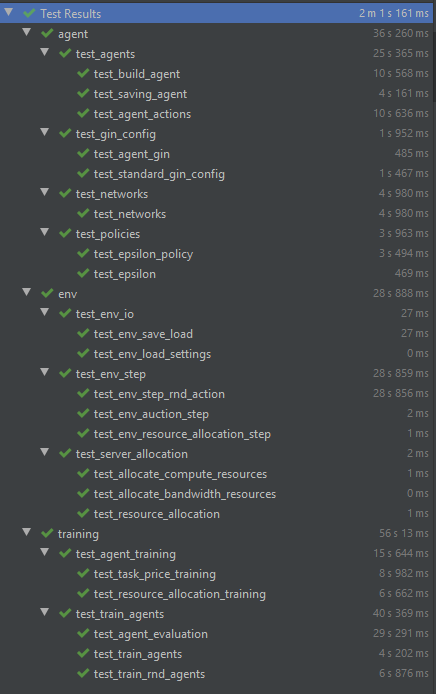
\includegraphics{figures/4_test_eval_figs/pytest_results.PNG}
    \caption{Results of the unit functions described in the Tables~\ref{tab:agent_testing},~\ref{tab:env_testing}
        and~\ref{tab:training_testing}}
    \label{fig:pytest_results}
\end{figure}

\section{Agent evaluation}\label{sec:agent-evaluation}
In order to compare the implemented agents from Chapter~\ref{ch:implementation-of-the-solution}, a range of metric are
used which are recorded while the agent is training. For the auction agent the metrics are: histogram winning prices,
number of no bids, number of failed tasks, number of completed tasks and a histogram of actions taken. For the resource
allocation agents the metrics are a histogram of weighting, number of failed tasks and number of completed tasks.
Using these metrics evaluation of agent performance can be done between the different reinforcement learning algorithms
implemented in Table~\ref{tab:reinforcement_learning_algorithms}, network architectures in
Table~\ref{tab:neural_network_layers} and methods of training different agents. \\
These evaluations fall into three families: env and agent num, algorithm and network architecture that are analysed in
Subsections~\ref{subsec:environment-and-agent-number-training},~\ref{subsec:reinforcement-learning-algorithm-training}
and~\ref{subsec:neural-network-architecture-training} respectively.

\subsection{Environment and Agent number training}\label{subsec:environment-and-agent-number-training}
The analysis of the different reinforcement learning algorithms and neural network architectures in
Subsection~\ref{subsec:reinforcement-learning-algorithm-training} and~\ref{subsec:neural-network-architecture-training}
respectively assume two qualities that this subsection analyses. These are the training and evaluation environments
and the number of agents used during training. As there are huge ranges of possible environment settings that agents
could be trained, investigating agent environment generality is a challenge and an important measure within machine
learning. This is of particular importance for this work, as in real-life, the environment that agents experiences will
can be unpredictable and different from those trained on. Meaning that agents should learn to generalise and not
overfit to particular environments used during training.

The other assume quality is due an advantage of the Vickrey auction over alternative auctions, explored in
Section~\ref{sec:auctioning-of-tasks}, that it is Incentive compatible. This auction property means that the dominant
strategy for all agents is to bid truthfully, which is the agent's true evaluation of the task. Therefore due to agents
not needing to learn to "out bid" each other allowing for effective self-play to be used in training.

Therefore this subsection compare the results of agents that are trained on a single environment setting and those
trained on multiple environment settings and when multiple or single agents are trained together.
These are compared using a set of pre-generated environments, one from the single environment setting and another from
the multiple environment settings.

%% Env training legend
\begin{wrapfigure}{r}{0.5\textwidth}
    \includegraphics[width=0.5\textwidth]{figures/4_test_eval_figs/env_training_fig/legend.png}
    \caption{Environment training legend}
    \label{fig:env-training-legend}
\end{wrapfigure}

During train, every 10 episodes, the agents are trained on the environments pre-generated from the multi-env settings.
Then in each of these evaluations, five metrics are collected: the number of completed tasks
(figure~\ref{fig:env_num_completed_tasks}), number of failed tasks (figure~\ref{fig:env_num_failed_tasks}),
the percentage of tasks attempted (figure~\ref{fig:env_percent_tasks}), total prices (figure~\ref{fig:env_total_prices})
and total winning prices (figure~\ref{fig:env_winning_prices}) when the environment are run. \\

%% Training evaluation
\begin{figure}[H]
    \centering
    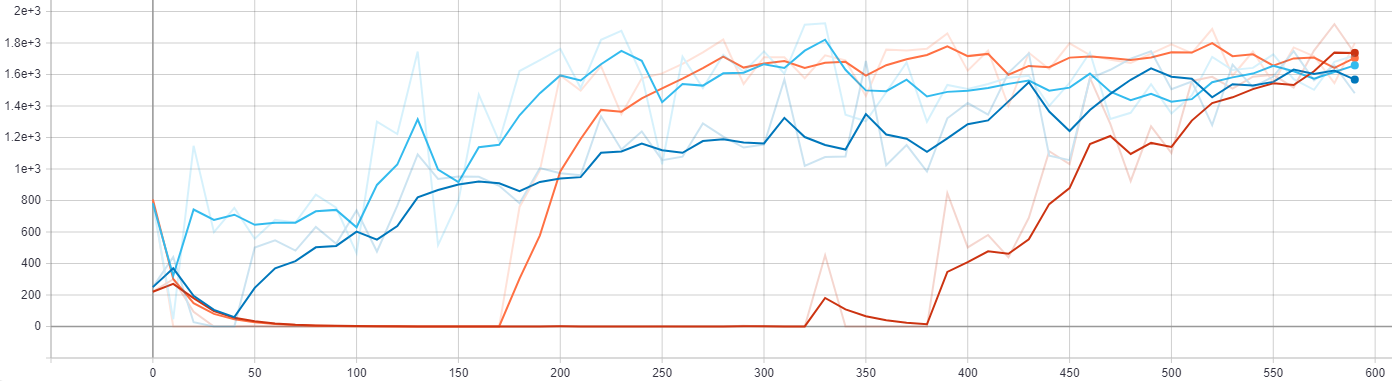
\includegraphics[width=17cm]{figures/4_test_eval_figs/env_training_fig/num_completed_tasks.png}
    \caption{Number of completed tasks}
    \label{fig:env_num_completed_tasks}
\end{figure}

\begin{figure}[H]
    \centering
    \includegraphics[width=17cm]{figures/4_test_eval_figs/env_training_fig/num_failed_tasks.png}
    \caption{Number of failed tasks}
    \label{fig:env_num_failed_tasks}
\end{figure}

\begin{figure}[H]
    \centering
    \includegraphics[width=17cm]{figures/4_test_eval_figs/env_training_fig/percent_tasks.png}
    \caption{Percentage of tasks attempted}
    \label{fig:env_percent_tasks}
\end{figure}

\begin{figure}[H]
    \centering
    \includegraphics[width=17cm]{figures/4_test_eval_figs/env_training_fig/total_prices.png}
    \caption{Total prices}
    \label{fig:env_total_prices}
\end{figure}

\begin{figure}[H]
    \centering
    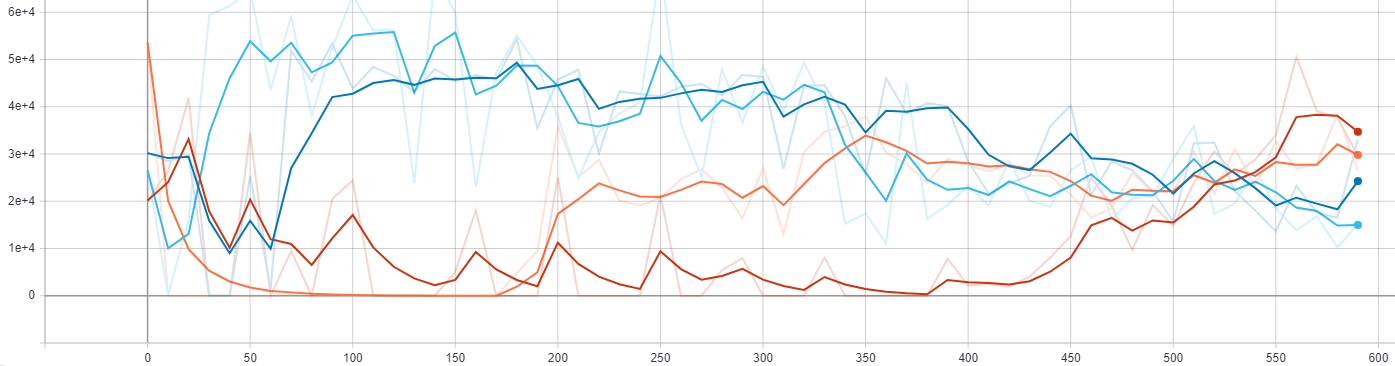
\includegraphics[width=17cm]{figures/4_test_eval_figs/env_training_fig/total_winning_prices.PNG}
    \caption{Total winning prices}
    \label{fig:env_winning_prices}
\end{figure}

%% Analysis of the training results
%% TODO

%% Auction prices and resource weightings histograms
%% TODO but Im not sure this is interesting or needed

\subsection{Reinforcement learning algorithm training}\label{subsec:reinforcement-learning-algorithm-training}
In table~\ref{tab:reinforcement_learning_algorithms}, a range of reinforcement learning algorithms were proposed as
methods of training neural networks. Using the analysis from the previous subsections, during training agents were
trained on multiple environment settings with multiple task pricing agents and a single resource weighting agents.
The evaluation environment were pre-generated as well to confirm uniform testing between the agents. \newline

\begin{wrapfigure}{l}{0.5\textwidth}
    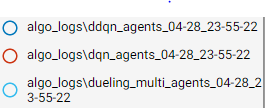
\includegraphics[width=0.5\textwidth]{figures/4_test_eval_figs/algo_training_fig/legend.PNG}
    \caption{Environment training legend}
    \label{fig:algo-training-legend}
\end{wrapfigure}

%% Training evaluation
\begin{figure}[H]
    \centering
    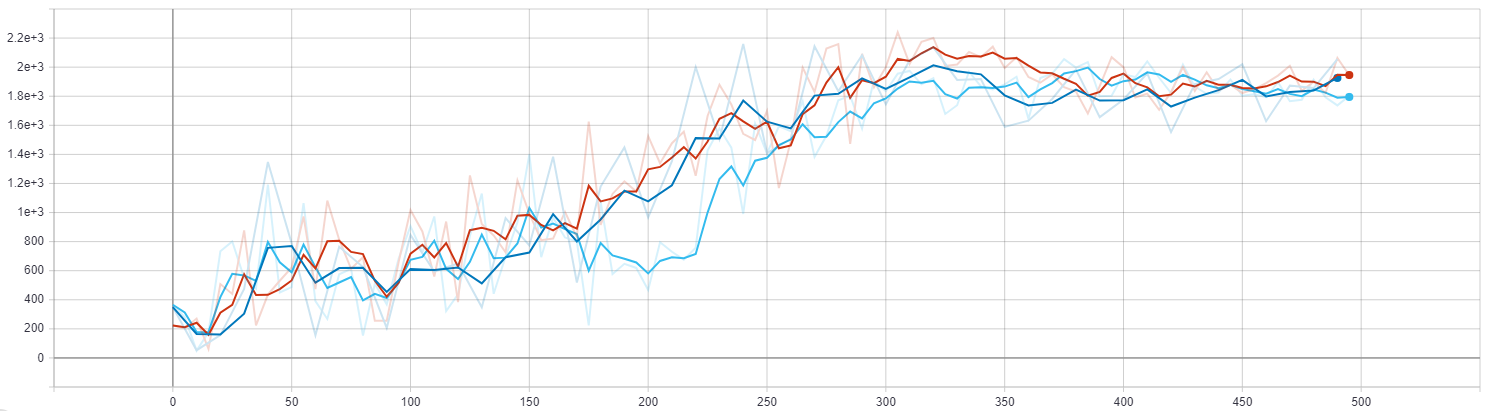
\includegraphics[width=17cm]{figures/4_test_eval_figs/algo_training_fig/num_completed_tasks.PNG}
    \caption{Number of completed tasks}
    \label{fig:algo_num_completed_tasks}
\end{figure}

\begin{figure}[H]
    \centering
    \includegraphics[width=17cm]{figures/4_test_eval_figs/algo_training_fig/num_failed_tasks.png}
    \caption{Number of failed tasks}
    \label{fig:algo_num_failed_tasks}
\end{figure}

\begin{figure}[H]
    \centering
    \includegraphics[width=17cm]{figures/4_test_eval_figs/algo_training_fig/percent_tasks.png}
    \caption{Percent of tasks attempted}
    \label{fig:algo_percent_tasks}
\end{figure}

\begin{figure}[H]
    \centering
    \includegraphics[width=17cm]{figures/4_test_eval_figs/algo_training_fig/total_prices.png}
    \caption{Total prices}
    \label{fig:algo_total_prices}
\end{figure}

\begin{figure}[H]
    \centering
    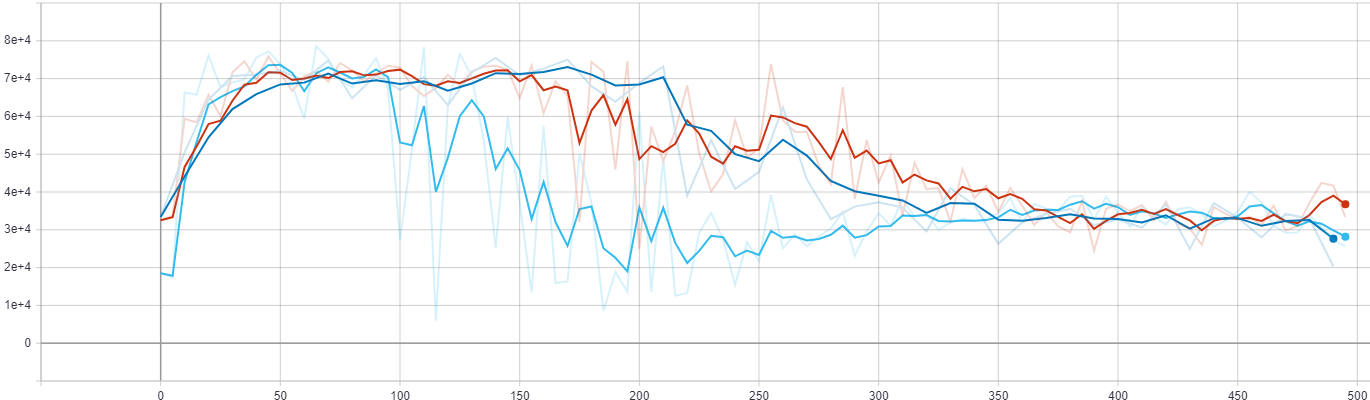
\includegraphics[width=17cm]{figures/4_test_eval_figs/algo_training_fig/total_winning_prices.PNG}
    \caption{Winning prices}
    \label{fig:algo_winning_prices}
\end{figure}

With the agents, an action histogram is recorded for all of the actions taken every 100 episodes to analyse the change
of actions taken over time and to investigate the difference is how algorithms evaluate the value of a position. Each
agent has the the auction and weighting actions separated due to their difference in policy. \newline

\begin{figure}[H]
    \centering
    \begin{minipage}{0.5\textwidth}
        \centering
        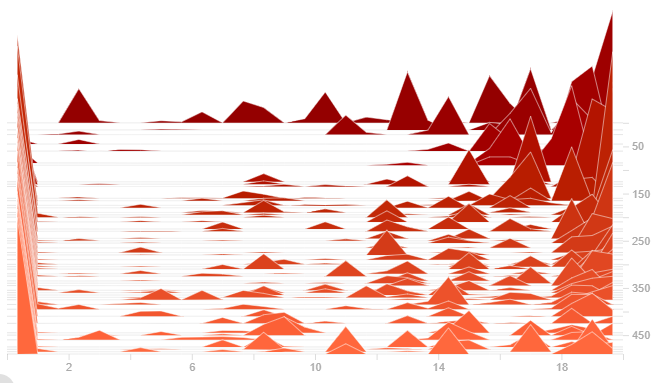
\includegraphics[width=1.0\textwidth]{figures/4_test_eval_figs/algo_training_fig/dqn_auction_prices.png}
        \caption{Deep Q Network auction prices}
        \label{fig:dqn-auction-prices}
    \end{minipage}\hfill
    \begin{minipage}{0.5\textwidth}
        \centering
        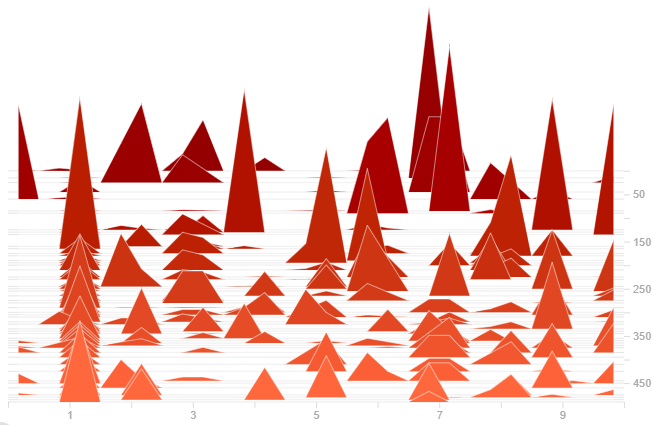
\includegraphics[width=1.0\textwidth]{figures/4_test_eval_figs/algo_training_fig/dqn_weightings.png}
        \caption{Deep Q Network resource weightings}
        \label{fig:dqn-resource-weightings}
    \end{minipage}
\end{figure}

\begin{figure}[H]
    \centering
    \begin{minipage}{0.5\textwidth}
        \centering
        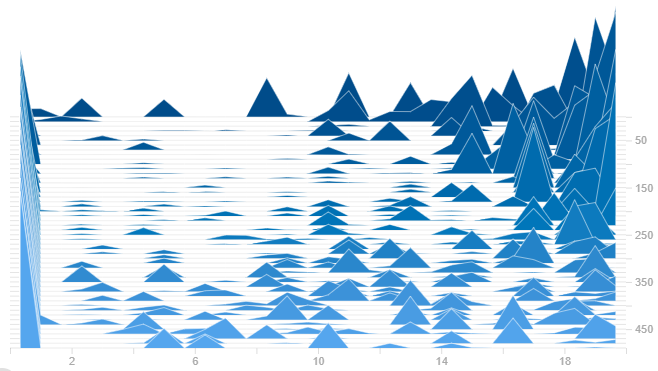
\includegraphics[width=1.0\textwidth]{figures/4_test_eval_figs/algo_training_fig/ddqn_auction_prices.png}
        \caption{Double Deep Q Network auction prices}
        \label{fig:ddqn-auction-prices}
    \end{minipage}\hfill
    \begin{minipage}{0.5\textwidth}
        \centering
        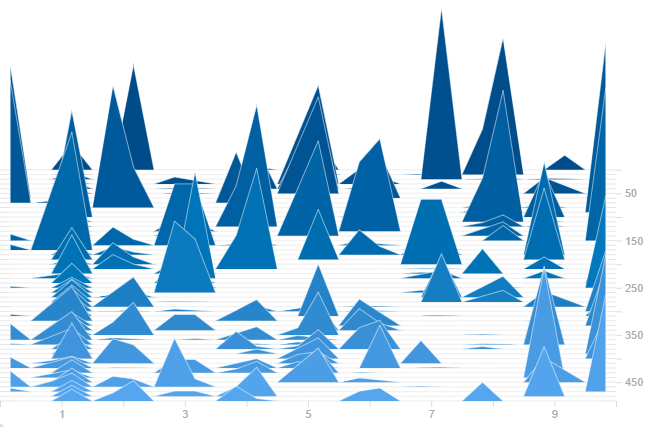
\includegraphics[width=1.0\textwidth]{figures/4_test_eval_figs/algo_training_fig/ddqn_weightings.png}
        \caption{Double Deep Q Network resource weightings}
        \label{fig:ddqn-resource-weightings}
    \end{minipage}
\end{figure}

\begin{figure}[H]
    \centering
    \begin{minipage}{0.5\textwidth}
        \centering
        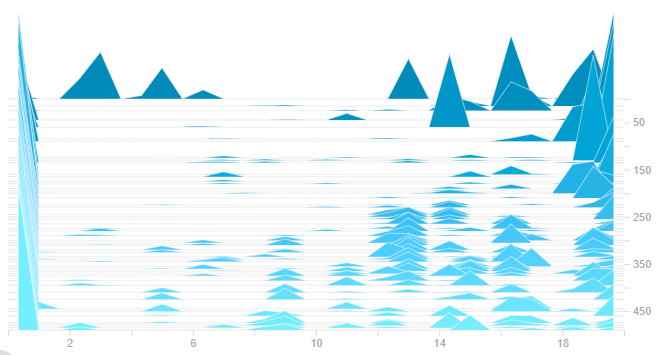
\includegraphics[width=1.0\textwidth]{figures/4_test_eval_figs/algo_training_fig/dueling_dqn_auction_prices.png}
        \caption{Dueling Deep Q Network auction prices}
        \label{fig:dueling-dqn-auction-prices}
    \end{minipage}\hfill
    \begin{minipage}{0.5\textwidth}
        \centering
        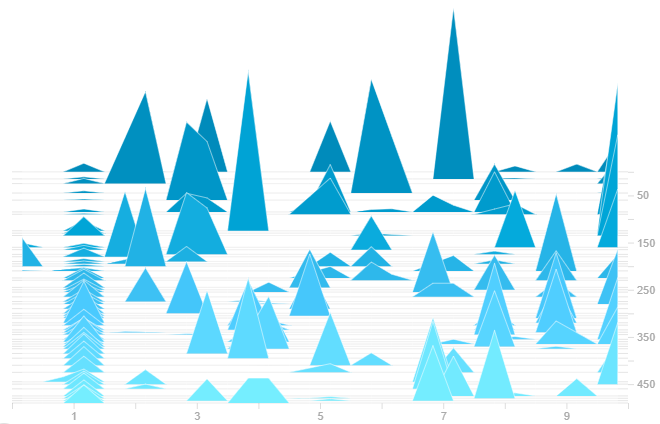
\includegraphics[width=1.0\textwidth]{figures/4_test_eval_figs/algo_training_fig/dueling_dqn_weightings.png}
        \caption{Dueling Deep Q Network resource weightings}
        \label{fig:dueling-dqn-resource-weightings}
    \end{minipage}
\end{figure}

\subsection{Neural network architecture training}\label{subsec:neural-network-architecture-training}
There are a wide-range of compatible neural network architectures that agents can use, as outlined in
table~\ref{tab:neural_network_layers}. To compare these architectures, the DQN agents from the previous subsection is
used due to its effectiveness and simplicity with four different network architectures: RNN~\citep{RNN},
LSTM~\citep{LSTM}, GRU~\citep{GRU} and Bidirectional~\citep{Bidirectional} using an LSTM network. \\

\begin{wrapfigure}{l}{0.5\textwidth}
    \includegraphics[width=0.5\textwidth]{figures/4_test_eval_figs/net_arch_training_fig/legend.png}
    \caption{Environment training legend}
    \label{fig:net-arch-training-legend}
\end{wrapfigure}

%% Training evaluation
\begin{figure}[H]
    \centering
    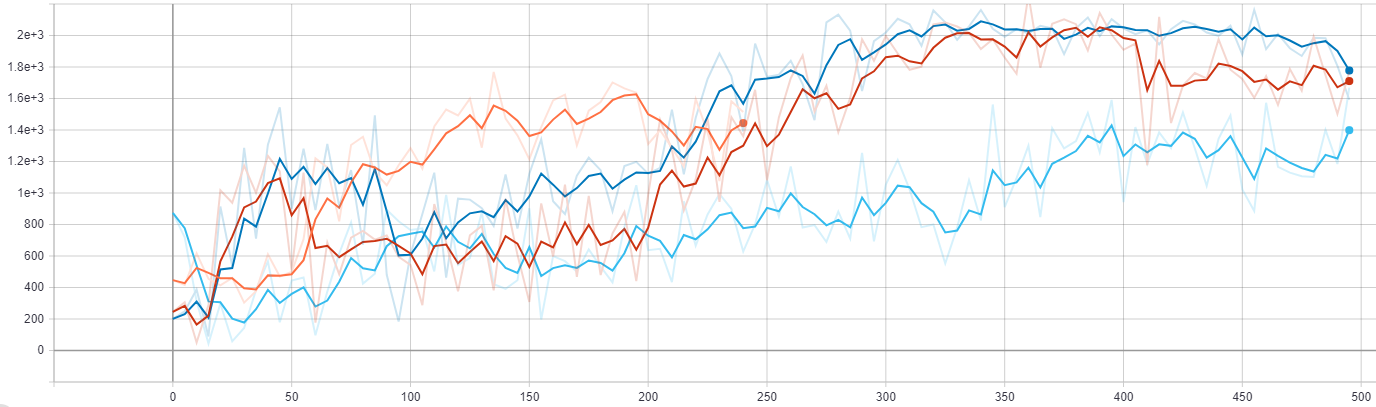
\includegraphics[width=17cm]{figures/4_test_eval_figs/net_arch_training_fig/num_completed_tasks.PNG}
    \caption{Number of completed tasks}
    \label{fig:net_arch_num_completed_tasks}
\end{figure}

\begin{figure}[H]
    \centering
    \includegraphics[width=17cm]{figures/4_test_eval_figs/net_arch_training_fig/num_failed_tasks.png}
    \caption{Number of failed tasks}
    \label{fig:net_arch_num_failed_tasks}
\end{figure}

\begin{figure}[H]
    \centering
    \includegraphics[width=17cm]{figures/4_test_eval_figs/net_arch_training_fig/percent_tasks.png}
    \caption{Percent of tasks attempted}
    \label{fig:net_arch_percent_tasks}
\end{figure}

\begin{figure}[H]
    \centering
    \includegraphics[width=17cm]{figures/4_test_eval_figs/net_arch_training_fig/total_prices.png}
    \caption{Total prices}
    \label{fig:net_arch_total_prices}
\end{figure}

%% TODO may not be needed
\begin{figure}[H]
    \centering
    \begin{minipage}{0.5\textwidth}
        \centering
        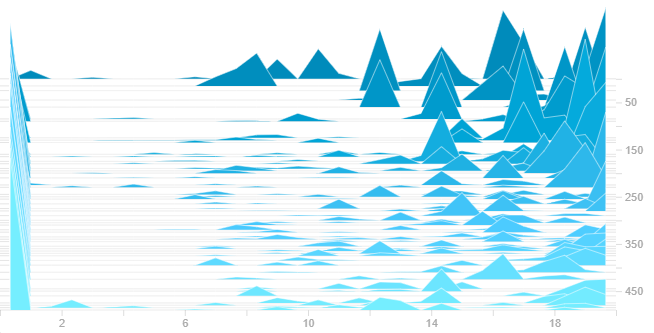
\includegraphics[width=1.0\textwidth]{figures/4_test_eval_figs/net_arch_training_fig/rnn_architecture_auction_prices.png}
        \caption{Rnn network architecture auction prices}
        \label{fig:rnn-auction-prices}
    \end{minipage}\hfill
    \begin{minipage}{0.5\textwidth}
        \centering
        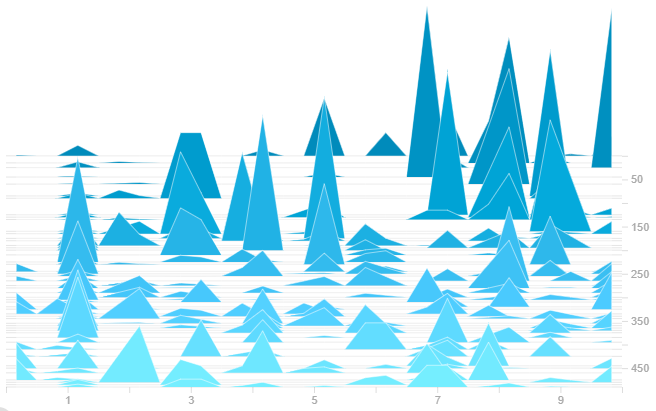
\includegraphics[width=1.0\textwidth]{figures/4_test_eval_figs/net_arch_training_fig/rnn_architecture_weightings.png}
        \caption{Rnn network architecture resource weightings}
        \label{fig:rnn-resource-weightings}
    \end{minipage}
\end{figure}

\begin{figure}[H]
    \centering
    \begin{minipage}{0.5\textwidth}
        \centering
        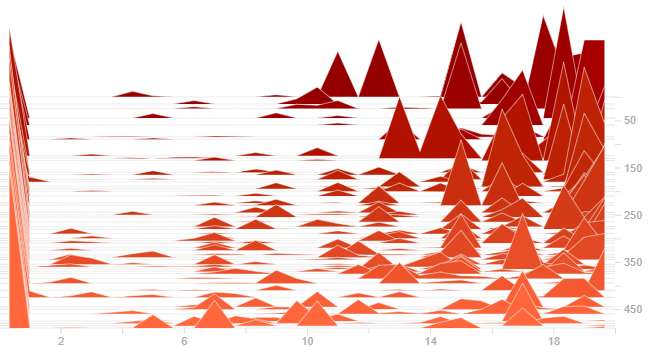
\includegraphics[width=1.0\textwidth]{figures/4_test_eval_figs/net_arch_training_fig/gru_architecture_auction_prices.png}
        \caption{GRU network architecture auction prices}
        \label{fig:gru-auction-prices}
    \end{minipage}\hfill
    \begin{minipage}{0.5\textwidth}
        \centering
        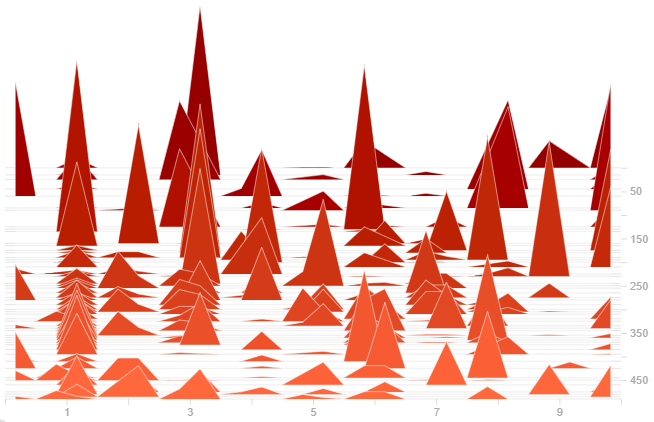
\includegraphics[width=1.0\textwidth]{figures/4_test_eval_figs/net_arch_training_fig/gru_architecture_weightings.png}
        \caption{GRU network architecture resource weightings}
        \label{fig:gru-resource-weightings}
    \end{minipage}
\end{figure}

\begin{figure}[H]
    \centering
    \begin{minipage}{0.5\textwidth}
        \centering
        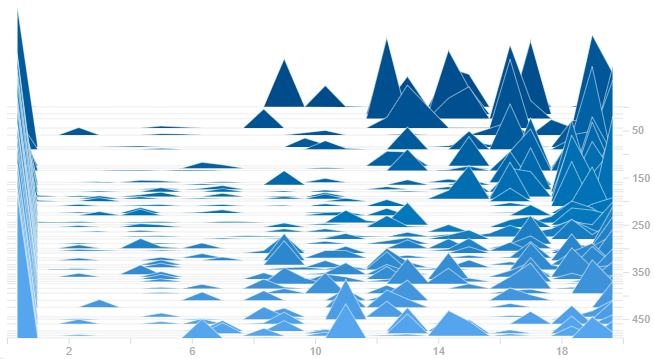
\includegraphics[width=1.0\textwidth]{figures/4_test_eval_figs/net_arch_training_fig/lstm_architecture_auction_prices.png}
        \caption{LSTM network architecture auction prices}
        \label{fig:lstm-auction-prices}
    \end{minipage}\hfill
    \begin{minipage}{0.5\textwidth}
        \centering
        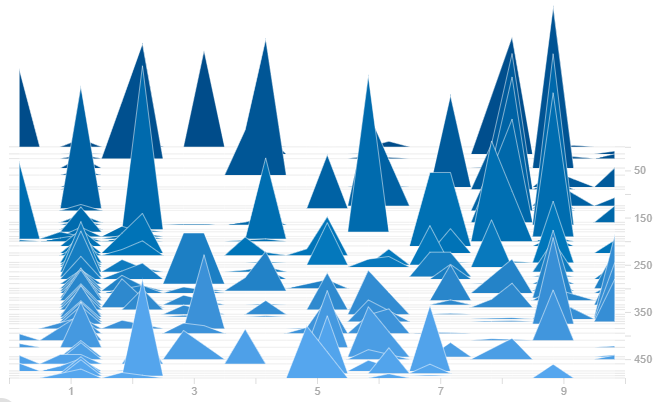
\includegraphics[width=1.0\textwidth]{figures/4_test_eval_figs/net_arch_training_fig/lstm_architecture_weightings.png}
        \caption{Rnn network architecture resource weightings}
        \label{fig:lstm-resource-weightings}
    \end{minipage}
\end{figure}

\begin{figure}[H]
    \centering
    \begin{minipage}{0.5\textwidth}
        \centering
        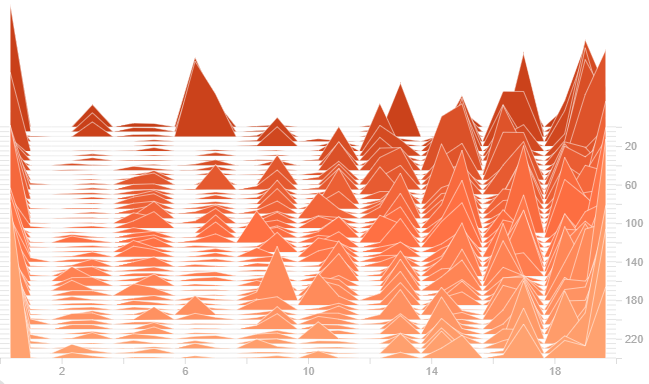
\includegraphics[width=1.0\textwidth]{figures/4_test_eval_figs/net_arch_training_fig/bidirectional_architecture_auction_prices.png}
        \caption{Bidirectional network architecture auction prices}
        \label{fig:bidirectional-auction-prices}
    \end{minipage}\hfill
    \begin{minipage}{0.5\textwidth}
        \centering
        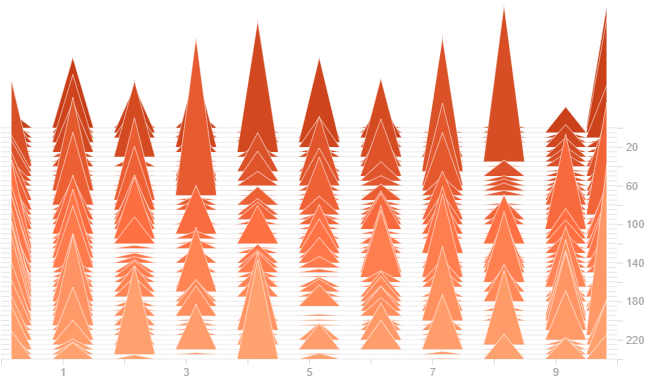
\includegraphics[width=1.0\textwidth]{figures/4_test_eval_figs/net_arch_training_fig/bidirectional_architecture_weightings.png}
        \caption{Bidirectional network architecture resource weightings}
        \label{fig:bidirectional-resource-weightings}
    \end{minipage}
\end{figure}